\PassOptionsToPackage{table}{xcolor}
\documentclass[aspectratio=169,10pt]{beamer}

% ── Theme ────────────────────────────────────────────────────────────────
\usetheme{Madrid}
\usecolortheme{whale}
\setbeamertemplate{navigation symbols}{}
\setbeamertemplate{footline}{
  \leavevmode\hbox{%
    \begin{beamercolorbox}[wd=.33\paperwidth,ht=2.5ex,dp=1ex,center]{author in head/foot}%
      \usebeamerfont{author in head/foot}\insertshortauthor
    \end{beamercolorbox}%
    \begin{beamercolorbox}[wd=.34\paperwidth,ht=2.5ex,dp=1ex,center]{title in head/foot}%
      \usebeamerfont{title in head/foot}\insertshorttitle
    \end{beamercolorbox}%
    \begin{beamercolorbox}[wd=.33\paperwidth,ht=2.5ex,dp=1ex,right]{date in head/foot}%
      \usebeamerfont{date in head/foot}\insertframenumber{}/\inserttotalframenumber\hspace*{2ex}
    \end{beamercolorbox}}%
}
\setbeamertemplate{section in toc}[sections numbered]
\setbeamertemplate{subsection in toc}[subsections numbered]
\setbeamercolor{block title}{bg=iitblue!85,fg=white}
\setbeamercolor{block body}{bg=iitblue!5}

% ── Packages ─────────────────────────────────────────────────────────────
\usepackage[utf8]{inputenc}
\usepackage[T1]{fontenc}
\usepackage{amsmath,amssymb}
\usepackage{booktabs}
\usepackage{multirow}
\usepackage{array}
\usepackage{tikz}
\usetikzlibrary{shapes.geometric,arrows,positioning,calc,fit,decorations.pathreplacing}
\usepackage{pgfplots}
\pgfplotsset{compat=1.18}
\usepackage{graphicx}
\usepackage{xcolor}

% ── Custom colors ────────────────────────────────────────────────────────
\definecolor{iitblue}{RGB}{0,51,102}
\definecolor{comp1}{RGB}{0,110,50}
\definecolor{comp2}{RGB}{180,30,30}
\definecolor{highlight}{RGB}{220,120,0}
\definecolor{soft}{RGB}{245,245,250}

% ── Custom commands ──────────────────────────────────────────────────────
\newcommand{\bho}{Bhojpuri}
\newcommand{\hi}{Hindi}
\newcommand{\xlmr}{XLM-RoBERTa}
\newcommand{\uas}{\textsc{uas}}
\newcommand{\las}{\textsc{las}}

% ── Title ────────────────────────────────────────────────────────────────
\title[Cross-Lingual Parsing for Bhojpuri]{Cross-Lingual Dependency Parsing for\\Low-Resource \bho{} via Parallel Bottleneck Adapters\\and Syntax-Aware Transfer}
\author[Kolgane S.\,S.]{Kolgane Sanskruti Sanjay\\{\small Roll No.\ 21074015}}
\institute[IIT (BHU)]{Department of Computer Science and Engineering\\Indian Institute of Technology (BHU), Varanasi\\[6pt]{\small Supervisor: \textbf{Dr.\ Anil Kumar Singh}}}
\date{26 April 2026}

\begin{document}

% ═══════════════════════════════════════════════════════════════════════
% SLIDE 1 --- TITLE
% ═══════════════════════════════════════════════════════════════════════
\begin{frame}[plain]
\titlepage
\end{frame}

% ═══════════════════════════════════════════════════════════════════════
% SLIDE 2 --- OUTLINE
% ═══════════════════════════════════════════════════════════════════════
\begin{frame}{Outline}
\vspace{0.3cm}
\begin{block}{\textcolor{comp1}{\textbf{Part 1 --- Novel Cross-Lingual Alignment}}}
\begin{itemize}
  \item Improving parser architecture on \hi{}--\bho{} aligned data
  \item \textbf{System F} (fine-tuning baseline) $\to$ \textbf{G} (MSE alignment) $\to$ \textbf{H} (SACT)
\end{itemize}
\end{block}

\vspace{0.3cm}
\begin{block}{\textcolor{comp2}{\textbf{Part 2 --- Real-World Benchmark Evaluation}}}
\begin{itemize}
  \item Parsing on the \bho{} Treebank (BHTB) --- the only gold benchmark
  \item \textbf{System A} (zero-shot baseline) $\to$ \textbf{K} (UD-Bridge self-training)
\end{itemize}
\end{block}

\vspace{0.3cm}
\centering\small
\emph{Part 1 builds the architecture; Part 2 applies the lessons to the real benchmark.}
\end{frame}

% ═══════════════════════════════════════════════════════════════════════
\section{Motivation and Background}
% ═══════════════════════════════════════════════════════════════════════

% SLIDE 3 --- DP IN ONE SLIDE
\begin{frame}{Dependency Parsing in One Slide}
\begin{columns}[T]
\column{0.52\textwidth}
\textbf{Task:} recover grammatical structure
\begin{itemize}
  \item Each word points to \textbf{one head}
  \item Each arc carries \textbf{one label}
  \item Output: a directed tree rooted at ROOT
\end{itemize}

\vspace{0.4cm}
\textbf{Why it matters:} feeds MT, QA, IE, semantic parsing.

\vspace{0.4cm}
\textbf{Evaluation:}
\begin{itemize}
  \item \textbf{\uas{}}: fraction of tokens with correct head
  \item \textbf{\las{}}: correct head \emph{and} correct label
\end{itemize}

\column{0.46\textwidth}
\centering
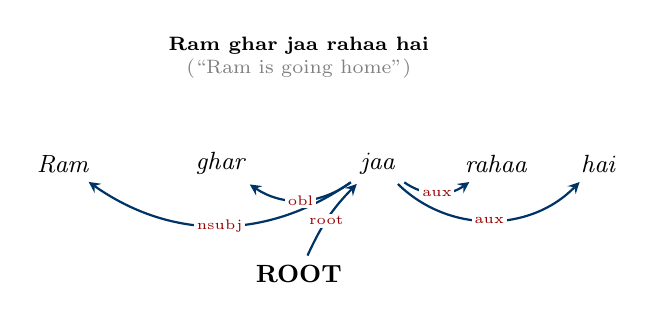
\begin{tikzpicture}[
  word/.style={font=\small\itshape},
  dep/.style={->,>=stealth,thick,iitblue},
  lbl/.style={font=\tiny,red!60!black,fill=white,inner sep=1pt}
]
\node[font=\scriptsize] at (0,3.1) {\textbf{Ram ghar jaa rahaa hai}};
\node[font=\scriptsize,gray] at (0,2.8) {(``Ram is going home'')};

\node[word] (ram)  at (-3,1.6) {Ram};
\node[word] (ghar) at (-1,1.6) {ghar};
\node[word] (jaa)  at ( 1,1.6) {jaa};
\node[word] (raha) at ( 2.5,1.6) {rahaa};
\node[word] (hai)  at ( 3.8,1.6) {hai};
\node[font=\small\bfseries] (root) at (0,0.2) {ROOT};

\draw[dep] (root) to[bend left=10] node[lbl,pos=0.45]{root} (jaa);
\draw[dep] (jaa) to[bend left=35] node[lbl]{nsubj} (ram);
\draw[dep] (jaa) to[bend left=35] node[lbl]{obl} (ghar);
\draw[dep] (jaa) to[bend right=35] node[lbl]{aux} (raha);
\draw[dep] (jaa) to[bend right=45] node[lbl]{aux} (hai);
\end{tikzpicture}
\end{columns}
\end{frame}

% SLIDE 4 --- WHY BHOJPURI
\begin{frame}{Why \bho{}? A Large Language, Almost No Tools}
\begin{columns}[T]
\column{0.58\textwidth}
\textbf{\bho{}:}
\begin{itemize}
  \item Eastern Indo-Aryan language, Devanagari script
  \item \textbf{50--60 million} native speakers
  \item Bihar, UP, Jharkhand + large diaspora
  \item Historically mislabelled as a ``Hindi dialect''
  \item ISO 639-3 code \texttt{bho} only since 2006
\end{itemize}

\vspace{0.3cm}
\begin{alertblock}{The challenge}
No large annotated \bho{} treebank exists $\Rightarrow$ we must \textbf{transfer from \hi{}}.
\end{alertblock}

\column{0.40\textwidth}
\begin{block}{Linguistic leverage}
\bho{} $\approx$ \hi{}:
\begin{itemize}\small
  \item Same SOV word order
  \item Shared vocabulary
  \item Shared Devanagari script
\end{itemize}
\end{block}

\vspace{0.3cm}
\begin{block}{What we have to work with}
\small
\begin{tabular}{@{}lr@{}}
\toprule
\textbf{Resource} & \textbf{Size} \\
\midrule
\hi{}--\bho{} aligned corpus & 30{,}966 pairs \\
\hi{} HDTB (UD)              & 13{,}304 sent \\
\bottomrule
\end{tabular}
\end{block}
\end{columns}
\end{frame}

% SLIDE 5 --- BUILDING BLOCKS
\begin{frame}{Building Blocks}
\begin{columns}[T]
\column{0.48\textwidth}
\textbf{\xlmr{} backbone}
\begin{itemize}
  \item 12 transformer layers, 768-dim
  \item Pretrained on 100 languages
  \item Includes \hi{} and \bho{} $\to$ shared Devanagari sub-word space
\end{itemize}

\vspace{0.3cm}
\textbf{Trankit toolkit}
\begin{itemize}
  \item End-to-end multilingual NLP pipeline
  \item Language-specific adapters
  \item Native biaffine parsing head
\end{itemize}

\column{0.48\textwidth}
\textbf{Pfeiffer adapters} (bottleneck $r=64$)
\begin{equation*}
\text{Adapter}(\mathbf{x})=\mathbf{x}+\mathbf{W}_{\text{up}}\,\phi(\mathbf{W}_{\text{down}}\,\text{LN}(\mathbf{x}))
\end{equation*}
\begin{itemize}
  \item Backbone \textbf{stays frozen}
  \item Only ${\sim}$100K params trained/language
  \item No catastrophic forgetting
\end{itemize}

\vspace{0.2cm}
\textbf{Biaffine scorer}
\begin{equation*}
s_{\text{arc}}(i,j)=\bigl(\mathbf{h}^{\text{dep}}_i\bigr)^{\!\top}\mathbf{W}\,\mathbf{h}^{\text{head}}_j
\end{equation*}
\end{columns}
\end{frame}

% ═══════════════════════════════════════════════════════════════════════
\section{Part 1: Novel Cross-Lingual Alignment}
% ═══════════════════════════════════════════════════════════════════════

% SLIDE 6 --- SYSTEM F
\begin{frame}{System F --- Warm-Start Fine-Tuning (Baseline)}
\begin{columns}[T]
\column{0.58\textwidth}
\textbf{Setup:} the straightforward approach.
\begin{itemize}
  \item Start from \hi{}-pretrained Trankit checkpoint
  \item Fine-tune \emph{all} parameters on 30{,}966 \hi{}--\bho{} aligned sentence pairs
  \item Standard supervised training with cross-entropy loss
\end{itemize}

\vspace{0.4cm}
\begin{block}{Dev Result}
\textbf{\uas{} 27.57\% \quad \las{} 17.75\%}
\end{block}

\vspace{0.3cm}
\textbf{Limitations:}
\begin{itemize}
  \item Full fine-tuning risks \emph{catastrophic forgetting} of multilingual prior
  \item No explicit cross-lingual alignment signal
  \item Updates ${\sim}$270M parameters for a small dataset
\end{itemize}

\column{0.40\textwidth}
\begin{alertblock}{Research question}
Can we do better than full fine-tuning by \emph{explicitly aligning} \hi{} and \bho{} representations?
\end{alertblock}

\vspace{0.3cm}
\begin{exampleblock}{Plan}
\textbf{G:} freeze backbone + representation-level alignment (MSE)\\[4pt]
\textbf{H:} replace MSE with syntax-aware losses (SACT)
\end{exampleblock}
\end{columns}
\end{frame}

% SLIDE 7 --- SYSTEM G
\begin{frame}{System G --- Parallel Adapters + MSE Alignment}
\begin{columns}[T]
\column{0.52\textwidth}
\textbf{First novel contribution.}

\vspace{0.2cm}
\textbf{Two design changes:}
\begin{enumerate}
  \item \textbf{Freeze \xlmr{}}; train only adapters + heads\\[-2pt]
        $\to$ no forgetting, $\sim$200K params total
  \item \textbf{MSE positional alignment}\\[-2pt]
        pull \bho{} hidden states toward \hi{} states at matched token positions
\end{enumerate}

\vspace{0.3cm}
\textbf{Training objective:}
\begin{equation*}
\mathcal{L}_G = \mathcal{L}_{\text{bho}} + 0.3\,\mathcal{L}_{\text{hi}} + 0.5\,\mathcal{L}_{\text{MSE}}
\end{equation*}

\vspace{0.2cm}
\begin{block}{Dev Result}
\textbf{\uas{} 55.70\% \quad \las{} 50.02\%}\\
\small \emph{$+32.3$ LAS over F, with 1000$\times$ fewer trainable params}
\end{block}

\column{0.45\textwidth}
\centering
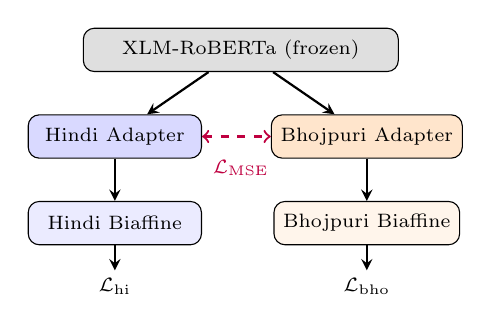
\begin{tikzpicture}[
  box/.style={rectangle,draw,rounded corners,minimum width=2.2cm,
              minimum height=0.55cm,text centered,font=\scriptsize},
  arrow/.style={->,>=stealth,thick}
]
\node[box,minimum width=4cm,fill=gray!25] (xlmr) at (0,0) {\xlmr{} (frozen)};
\node[box,fill=blue!15]   (ha) at (-1.6,-1.1) {\hi{} Adapter};
\node[box,fill=orange!20] (ba) at ( 1.6,-1.1) {\bho{} Adapter};
\node[box,fill=blue!8]    (hh) at (-1.6,-2.2) {\hi{} Biaffine};
\node[box,fill=orange!8]  (bh) at ( 1.6,-2.2) {\bho{} Biaffine};
\node[font=\scriptsize] at (-1.6,-3.0) {$\mathcal{L}_{\text{hi}}$};
\node[font=\scriptsize] at ( 1.6,-3.0) {$\mathcal{L}_{\text{bho}}$};
\node[font=\scriptsize,purple] at (0,-1.5) {$\mathcal{L}_{\text{MSE}}$};

\draw[arrow] (xlmr) -- (ha);
\draw[arrow] (xlmr) -- (ba);
\draw[arrow] (ha) -- (hh);
\draw[arrow] (ba) -- (bh);
\draw[arrow] (hh) -- +(0,-0.6);
\draw[arrow] (bh) -- +(0,-0.6);
\draw[<->,dashed,thick,purple] (ha) -- (ba);
\end{tikzpicture}
\end{columns}
\end{frame}

% SLIDE 8 --- SYSTEM H (SACT)
\begin{frame}{System H --- SACT: Syntax-Aware Cross-Lingual Transfer}
\textbf{Refined novel contribution.} MSE aligns \emph{representations uniformly}; SACT replaces it with \emph{three syntax-aware objectives}.

\vspace{0.25cm}
\begin{columns}[T]
\column{0.32\textwidth}
\begin{block}{1. Content-word cosine}
\begin{itemize}\small
  \item Scale-invariant alignment
  \item Nouns/verbs: weight $1.5$
  \item Function words: weight $0.3$
  \item Focus on syntactic anchors
\end{itemize}
\end{block}

\column{0.32\textwidth}
\begin{block}{2. Arc-KL distillation}
\begin{itemize}\small
  \item \hi{} parser = teacher
  \item Transfer parsing \emph{decisions}, not just representations
  \item KL on arc-score distributions
\end{itemize}
\end{block}

\column{0.32\textwidth}
\begin{block}{3. Cross-lingual Tree Supervision}
\begin{itemize}\small
  \item Matched token pairs
  \item \hi{} gold heads re-used for \bho{}
  \item Doubles structural signal
  \item Clean, not auto-transferred
\end{itemize}
\end{block}
\end{columns}

\vspace{0.3cm}
\begin{equation*}
\mathcal{L}_H = \mathcal{L}_{\text{bho}}
 + 0.5\,\mathcal{L}_{\text{hi}}
 + 0.4\,\mathcal{L}_{\text{cos}}
 + 2.0\,\mathcal{L}_{\text{arc-kl}}
 + 0.2\,\mathcal{L}_{\text{cts}}
\end{equation*}

\vspace{0.2cm}
\centering
\colorbox{comp1!18}{\textbf{Dev: \uas{} 55.85\% \quad \las{} 50.08\% \quad --- my best architecture on aligned data}}
\end{frame}

% SLIDE 9 --- PART 1 RESULTS
\begin{frame}{Results on \hi{}--\bho{} Aligned Dev Set}
\centering
\begin{tabular}{@{}llcc@{}}
\toprule
\textbf{System} & \textbf{Method} & \textbf{Dev UAS} & \textbf{Dev LAS} \\
\midrule
F & Warm-start fine-tuning (baseline)    & 27.57 & 17.75 \\
G & Parallel Adapters + MSE (novel \#1)   & 55.70 & 50.02 \\
\rowcolor{comp1!15}
\textbf{H} & \textbf{SACT --- Cosine + Arc-KL + CTS (novel \#2)} & \textbf{55.85} & \textbf{50.08} \\
\bottomrule
\end{tabular}

\vspace{0.8cm}
\begin{columns}[T]
\column{0.5\textwidth}
\textbf{Key observations}
\begin{itemize}\small
  \item Freezing \xlmr{} (G vs.\ F) eliminates forgetting
  \item Syntax-aware losses (H vs.\ G) beat uniform MSE
  \item SACT converges \emph{much faster} (next slide)
\end{itemize}

\column{0.5\textwidth}
\textbf{Head-to-head (\las{} gain)}
\begin{itemize}\small
  \item F $\to$ G: \textbf{+32.3\%} (frozen backbone + MSE)
  \item G $\to$ H: \textbf{+0.06\%} at convergence
  \item G $\to$ H: \textbf{+3.3\%} at epoch 1
\end{itemize}
\end{columns}

\vspace{0.4cm}
\centering
\colorbox{comp1!15}{\textbf{Both novel designs (G, H) beat the naive fine-tuning baseline (F).}}
\end{frame}

% SLIDE 10 --- LEARNING CURVES
\begin{frame}{Learning Curves: G vs.\ H}
\centering
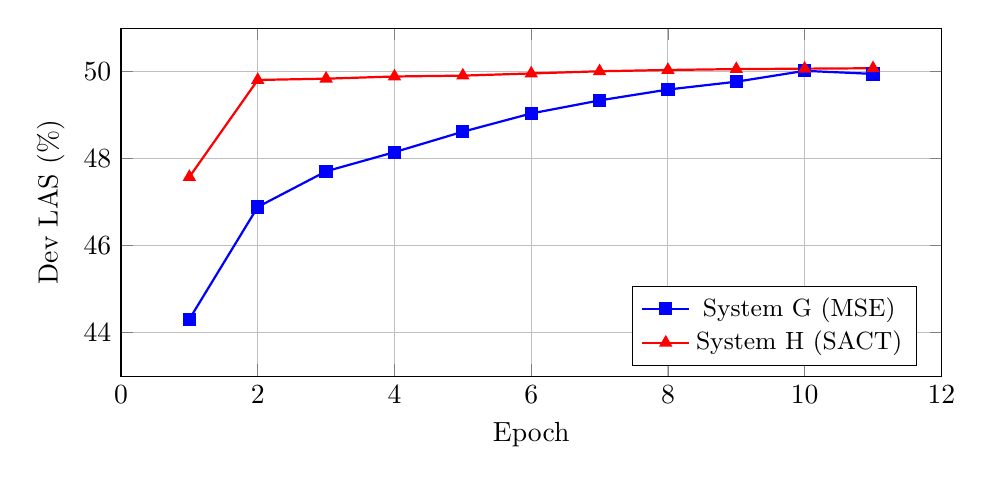
\begin{tikzpicture}
\begin{axis}[
  width=12cm, height=6cm,
  xlabel={Epoch},
  ylabel={Dev LAS (\%)},
  legend pos=south east,
  grid=major,
  xmin=0, xmax=12,
  ymin=43, ymax=51,
  legend style={font=\small},
]
\addplot[blue,thick,mark=square*,mark size=2] coordinates {
  (1,44.31) (2,46.89) (3,47.71) (4,48.15) (5,48.62) (6,49.04) (7,49.34) (8,49.59) (9,49.77) (10,50.02) (11,49.95)
};
\addlegendentry{System G (MSE)}

\addplot[red,thick,mark=triangle*,mark size=2] coordinates {
  (1,47.58) (2,49.81) (3,49.84) (4,49.89) (5,49.91) (6,49.96) (7,50.01) (8,50.04) (9,50.06) (10,50.07) (11,50.08)
};
\addlegendentry{System H (SACT)}
\end{axis}
\end{tikzpicture}

\vspace{0.1cm}
\small System H starts \textbf{+3.3 \las{}} ahead at epoch 1 and reaches near-final performance by epoch 2
--- syntax-aware losses give stronger gradient signal from the start.
\end{frame}

% SLIDE 11 --- ABLATION
\begin{frame}{Ablation --- What Does Each SACT Component Contribute?}
\centering
\begin{tabular}{@{}lcc c@{}}
\toprule
\textbf{Configuration} & \textbf{Dev UAS} & \textbf{Dev LAS} & $\Delta$\las{} \\
\midrule
Full System H                    & \textbf{55.85} & \textbf{50.08} & --- \\
\quad $-$ CTS                    & 55.64 & 49.87 & $-0.21$ \\
\quad $-$ Arc-KL distillation    & 55.71 & 49.94 & $-0.14$ \\
\quad $-$ Cosine alignment       & 55.48 & 49.71 & $-0.37$ \\
\quad $-$ \hi{} loss             & 55.39 & 49.62 & $-0.46$ \\
\quad $-$ All auxiliary losses   & 54.21 & 48.93 & $-1.15$ \\
\bottomrule
\end{tabular}

\vspace{0.6cm}
\textbf{Contribution ranking (by \las{} drop when removed):}
\begin{enumerate}
  \item \hi{} regularisation: $+0.46\%$
  \item Cosine alignment: $+0.37\%$
  \item Cross-lingual Tree Supervision: $+0.21\%$
  \item Arc-KL distillation: $+0.14\%$
\end{enumerate}

\centering
\vspace{0.1cm}
\emph{All four auxiliary signals contribute positively; none is redundant.}
\end{frame}

% SLIDE 12 --- PART 1 TAKEAWAY
\begin{frame}{Part 1 Takeaway}
\vspace{0.5cm}
\begin{center}
\colorbox{comp1!15}{\parbox{0.85\textwidth}{\centering\large
\textbf{My novel cross-lingual alignment losses improve over naive fine-tuning on the \hi{}--\bho{} aligned corpus.}
}}
\end{center}

\vspace{0.7cm}
\begin{columns}[T]
\column{0.48\textwidth}
\textbf{What worked}
\begin{itemize}
  \item Freezing the backbone (G, H) $>$ full FT (F)
  \item Syntax-aware supervision (H) $>$ uniform MSE (G)
  \item Faster convergence with SACT
\end{itemize}

\column{0.48\textwidth}
\textbf{Architectural progression}
\[
\text{F}\;\xrightarrow{\text{freeze}+\text{MSE}}\;\text{G}\;\xrightarrow{\text{syntax-aware}}\;\text{H}
\]
\vspace{0.1cm}
+32.3\%~\las{} \hfill +0.06\%~\las{} @ convergence\\
\phantom{+32.3\%~\las{}} \hfill +3.3\%~\las{} @ epoch 1
\end{columns}

\vspace{0.6cm}
\centering
\small \textit{Aligned-data performance is one story --- but the real benchmark for \bho{} lies elsewhere.}
\end{frame}

% ═══════════════════════════════════════════════════════════════════════
\section{Part 2: Real-World Benchmark Evaluation}
% ═══════════════════════════════════════════════════════════════════════

% SLIDE 13 --- BHTB INTRO + SCHEMA MISMATCH
\begin{frame}{The \bho{} Treebank (BHTB) --- The Real Benchmark}
\begin{columns}[T]
\column{0.48\textwidth}
\textbf{BHTB:} the only gold \bho{} treebank.
\begin{itemize}
  \item \textbf{357} manually annotated sentences
  \item Strict \textbf{Universal Dependencies (UD)} schema
  \item Test-only set --- the standard evaluation for \bho{} parsing
\end{itemize}

\vspace{0.3cm}
\textbf{Why can't we just use Systems F/G/H?}
\begin{itemize}
  \item Aligned corpus uses \emph{auto-transferred} labels
  \item Multiple roots, cycles, non-UD relations
  \item BHTB uses \emph{strict UD} labels
  \item \textbf{Label inventories don't match} $\Rightarrow$ training signal in wrong space
\end{itemize}

\column{0.48\textwidth}
\centering
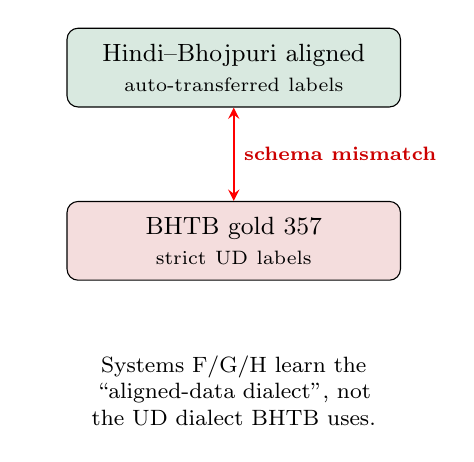
\begin{tikzpicture}[
  box/.style={rectangle,draw,rounded corners,align=center,text width=4cm,
              minimum height=1.0cm,font=\small},
  lbl/.style={font=\scriptsize\itshape}
]
\node[box,fill=comp1!15] (aligned) at (0,2)   {\hi{}--\bho{} aligned\\{\scriptsize auto-transferred labels}};
\node[box,fill=comp2!15] (bhtb)    at (0,-0.2) {BHTB gold 357\\{\scriptsize strict UD labels}};
\draw[<->,thick,red,>=stealth] (aligned) -- node[right,font=\scriptsize,red!80!black]{\textbf{schema mismatch}} (bhtb);

\node[font=\footnotesize,align=center,text width=5cm] at (0,-2.1) {Systems F/G/H learn the\\``aligned-data dialect'', not\\the UD dialect BHTB uses.};
\end{tikzpicture}
\end{columns}

\vspace{0.4cm}
\centering
\colorbox{yellow!30}{\parbox{0.85\textwidth}{\centering\small
To compete on BHTB, we need a parser trained \emph{in the UD label space} --- a different strategy from Part 1.
}}
\end{frame}

% SLIDE 14 --- SYSTEM A
\begin{frame}{System A --- Zero-Shot Baseline on BHTB}
\begin{columns}[T]
\column{0.55\textwidth}
\textbf{Idea:} rely on \xlmr{}'s shared multilingual space.
\begin{itemize}
  \item Train Trankit on \textbf{\hi{} HDTB} (13{,}304 UD sentences)
  \item Apply \emph{directly} to \bho{} --- no \bho{} training at all
  \item Labels automatically live in UD space (HDTB is native UD)
\end{itemize}

\vspace{0.4cm}
\begin{block}{BHTB gold result}
\textbf{\uas{} 52.78\% \quad \las{} 35.36\%}
\end{block}

\vspace{0.3cm}
\textcolor{comp2}{\textbf{This is the baseline to beat.}}\\[4pt]
A reasonable score without a single labelled \bho{} sentence --- purely from \hi{}-to-\bho{} transfer via \xlmr{}.

\column{0.42\textwidth}
\centering
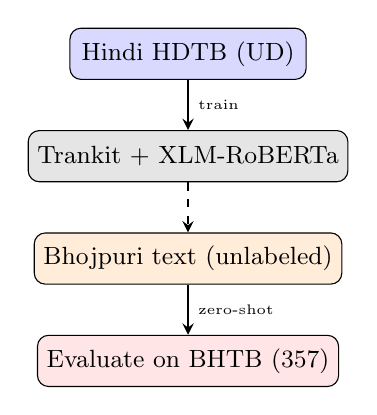
\begin{tikzpicture}[
  box/.style={rectangle,draw,rounded corners,minimum width=3cm,
              minimum height=0.65cm,text centered,font=\small},
  arrow/.style={->,>=stealth,thick}
]
\node[box,fill=blue!15]   (hdtb)    at (0, 2.6) {\hi{} HDTB (UD)};
\node[box,fill=gray!20]   (trankit) at (0, 1.3) {Trankit + \xlmr{}};
\node[box,fill=orange!15] (bho)     at (0, 0.0) {\bho{} text (unlabeled)};
\node[box,fill=red!10]    (bhtb)    at (0,-1.3) {Evaluate on BHTB (357)};

\draw[arrow] (hdtb) -- node[right,font=\tiny]{train} (trankit);
\draw[arrow,dashed] (trankit) -- (bho);
\draw[arrow] (bho) -- node[right,font=\tiny]{zero-shot} (bhtb);
\end{tikzpicture}
\end{columns}
\end{frame}

% SLIDE 15 --- SYSTEM K
\begin{frame}{System K --- UD-Bridge via Silver Self-Training}

\textbf{Novel contribution for the \bho{} benchmark.}\\[2pt]
\textit{Premise:} schema consistency beats data quantity when evaluating on BHTB.

\vspace{0.25cm}
\begin{center}
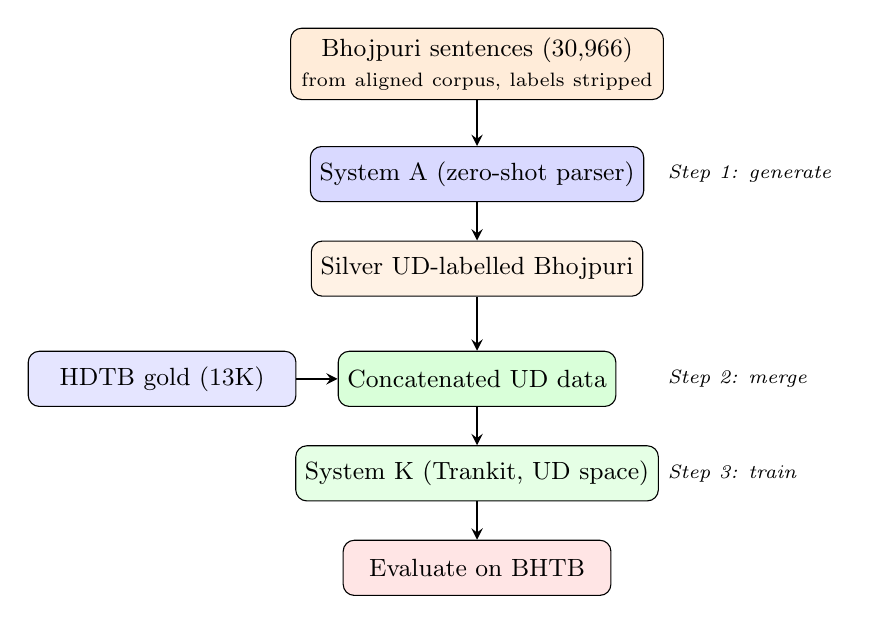
\begin{tikzpicture}[
  box/.style={rectangle,draw,rounded corners,minimum width=3.4cm,
              minimum height=0.7cm,text centered,font=\small},
  arrow/.style={->,>=stealth,thick},
  stepnum/.style={font=\scriptsize\itshape,right}
]
\node[box,fill=orange!15,align=center,text width=4.5cm] (bhotokens) at (0, 3.0) {\bho{} sentences (30{,}966)\\{\scriptsize from aligned corpus, labels stripped}};
\node[box,fill=blue!15]   (sysa)      at (0, 1.6) {System A (zero-shot parser)};
\node[box,fill=orange!10] (silver)    at (0, 0.4) {Silver UD-labelled \bho{}};
\node[stepnum] at (2.3,1.6) {Step 1: generate};

\node[box,fill=blue!10]  (hdtb)   at (-4,-1.0) {HDTB gold (13K)};
\node[box,fill=green!15] (concat) at (0,-1.0) {Concatenated UD data};
\node[stepnum] at (2.3,-1.0) {Step 2: merge};

\node[box,fill=green!10] (sysk) at (0,-2.2) {System K (Trankit, UD space)};
\node[box,fill=red!10]   (eval) at (0,-3.4) {Evaluate on BHTB};
\node[stepnum] at (2.3,-2.2) {Step 3: train};

\draw[arrow] (bhotokens) -- (sysa);
\draw[arrow] (sysa) -- (silver);
\draw[arrow] (silver) -- (concat);
\draw[arrow] (hdtb) -- (concat);
\draw[arrow] (concat) -- (sysk);
\draw[arrow] (sysk) -- (eval);
\end{tikzpicture}
\end{center}

\vspace{0.1cm}
\centering
\colorbox{comp2!15}{\textbf{Result: K surpasses A on BHTB --- 54.27\% \uas{} / 36.70\% \las{}}}
\end{frame}

% SLIDE 16 --- WHY UD-BRIDGE WORKS
\begin{frame}{Why UD-Bridge Works}
\begin{columns}[T]
\column{0.48\textwidth}
\textbf{The schema-consistency argument}
\begin{itemize}
  \item System A already parses in UD space (from HDTB)
  \item Its silver \bho{} labels are \emph{noisy but schema-consistent}
  \item Adding HDTB gold alongside \emph{regularises} training and anchors structure
  \item Any improvement on the training objective transfers directly to BHTB
\end{itemize}

\column{0.48\textwidth}
\textbf{What makes silver data good enough?}
\begin{itemize}
  \item Not every silver label is correct
  \item But errors are \emph{random}, not \emph{systematic schema errors}
  \item Gold HDTB supervision pulls silver noise toward correct UD patterns
  \item No mismatch between training and test schemas
\end{itemize}
\end{columns}

\vspace{0.7cm}
\begin{center}
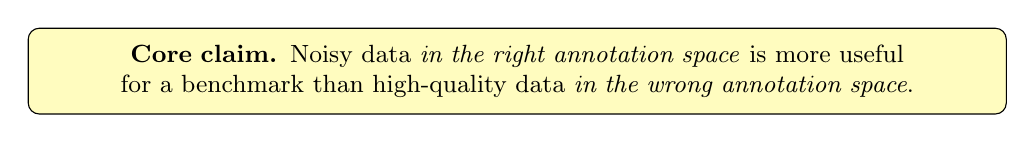
\begin{tikzpicture}
\node[draw,rounded corners,fill=yellow!25,text width=12cm,align=center,font=\small,inner sep=6pt] {
\textbf{Core claim.} Noisy data \emph{in the right annotation space} is more useful for a benchmark than high-quality data \emph{in the wrong annotation space}.
};
\end{tikzpicture}
\end{center}
\end{frame}

% SLIDE 17 --- PART 2 RESULTS
\begin{frame}{Results on BHTB Gold}
\centering
\begin{tabular}{@{}llcc@{}}
\toprule
\textbf{System} & \textbf{Method} & \textbf{BHTB UAS} & \textbf{BHTB LAS} \\
\midrule
A & Zero-shot Trankit (\hi{} HDTB only) --- baseline     & 52.78 & 35.36 \\
\rowcolor{comp2!15}
\textbf{K} & \textbf{UD-Bridge silver self-training (novel)} & \textbf{54.27} & \textbf{36.70} \\
\bottomrule
\end{tabular}

\vspace{0.8cm}
\textbf{Why K wins}
\begin{itemize}
  \item Adds \bho{}-specific supervision that System A never saw
  \item Keeps training + test labels in the same UD schema
  \item HDTB gold prevents silver noise from dominating
\end{itemize}

\vspace{0.5cm}
\centering
\colorbox{comp2!15}{\textbf{K beats A by +1.49\% \uas{} / +1.34\% \las{} $\Rightarrow$ state-of-the-art on real \bho{} parsing.}}
\end{frame}

% SLIDE 18 --- ERROR ANALYSIS
\begin{frame}{Error Analysis --- Where the Parser Wins and Loses}
\centering
\small
\begin{tabular}{@{}lrrr @{\hspace{1cm}} lrrr@{}}
\toprule
\multicolumn{4}{c}{\textbf{Structural / Local}} & \multicolumn{4}{c}{\textbf{Clausal / Long-range}} \\
\textbf{Rel} & \textbf{Corr} & \textbf{Tot} & \textbf{\las{}} &
\textbf{Rel} & \textbf{Corr} & \textbf{Tot} & \textbf{\las{}} \\
\midrule
case    & 755 & 907   & \textbf{83.2\%} &  acl    &  1 & 105 & 1.0\% \\
root    & 177 & 357   & 49.6\% &  advcl  &  3 &  82 & 3.7\% \\
punct   & 317 & 695   & 45.6\% &  xcomp  &  0 &  67 & 0.0\% \\
mark    &  52 & 123   & 42.3\% &  ccomp  &  0 &  58 & 0.0\% \\
amod    &  74 & 202   & 36.6\% &  cc     &  1 &  30 & 3.3\% \\
nmod    & 261 & 907   & 28.8\% &  obj    & 18 & 122 & 14.8\% \\
\bottomrule
\end{tabular}

\vspace{0.5cm}
\begin{columns}[T]
\column{0.5\textwidth}
\textbf{Transfers well}
\begin{itemize}\small
  \item Local, short-arc relations
  \item Morphologically marked (case, adp.)
  \item Consistent between \hi{} and \bho{}
\end{itemize}

\column{0.5\textwidth}
\textbf{Breaks down}
\begin{itemize}\small
  \item Clause-level relations (xcomp, ccomp, acl, advcl)
  \item Word-order-sensitive
  \item Where \bho{} diverges syntactically from \hi{}
\end{itemize}
\end{columns}
\end{frame}

% SLIDE 19 --- PART 2 TAKEAWAY
\begin{frame}{Part 2 Takeaway}
\vspace{0.5cm}
\begin{center}
\colorbox{comp2!15}{\parbox{0.85\textwidth}{\centering\large
\textbf{UD-Bridge self-training beats the zero-shot baseline on BHTB --- advancing state-of-the-art on the real \bho{} parsing benchmark.}
}}
\end{center}

\vspace{0.7cm}
\begin{columns}[T]
\column{0.48\textwidth}
\textbf{What made the difference}
\begin{itemize}
  \item Train and test share the same UD schema
  \item Silver \bho{} data adds language-specific signal
  \item HDTB gold anchors correct UD structure
\end{itemize}

\column{0.48\textwidth}
\textbf{The bigger methodological lesson}
\begin{itemize}
  \item Schema consistency matters as much as model quality
  \item ``Noisy but correctly-labelled'' $>$ ``clean but mislabelled''
  \item Self-training is a clean bridge into low-resource UD settings
\end{itemize}
\end{columns}
\end{frame}

% ═══════════════════════════════════════════════════════════════════════
\section{Conclusion}
% ═══════════════════════════════════════════════════════════════════════

% SLIDE 20 --- KEY FINDINGS
\begin{frame}{Key Findings Across Both Parts}
\begin{enumerate}
  \item \textbf{Freezing the backbone is essential.}\\
        Full fine-tuning (F) on cross-lingual transferred labels causes catastrophic forgetting.
        Adapters preserve the multilingual prior with $\sim$200K params.

  \vspace{0.25cm}
  \item \textbf{Syntax-aware alignment beats representation alignment.}\\
        SACT's Arc-KL and CTS supervise parsing \emph{decisions} directly ---
        stronger and faster gradient signal than uniform MSE.

  \vspace{0.25cm}
  \item \textbf{Schema consistency matters as much as model quality.}\\
        Strong aligned-data performance does not automatically translate to benchmark gains.
        Training signal must live in the same annotation space as the test set.

  \vspace{0.25cm}
  \item \textbf{Self-training bridges low-resource settings cleanly.}\\
        UD-Bridge's silver-from-zero-shot approach adds language-specific
        supervision while keeping schema alignment intact.
\end{enumerate}
\end{frame}

% SLIDE 21 --- CONTRIBUTIONS
\begin{frame}{Contributions}
\textbf{Novel architectural contributions (Part 1):}
\begin{enumerate}
  \item \textbf{System G} --- parallel adapter architecture with frozen \xlmr{} + MSE alignment
  \item \textbf{System H (SACT)} --- three syntax-aware alignment losses
        (content-word cosine, Arc-KL distillation, Cross-lingual Tree Supervision)\\
        \textbf{Best \las{}: 50.08\% on \hi{}--\bho{} aligned Dev}
\end{enumerate}

\vspace{0.4cm}
\textbf{Novel benchmark contribution (Part 2):}
\begin{enumerate}\setcounter{enumi}{2}
  \item \textbf{System K (UD-Bridge)} --- silver self-training for schema-consistent
        training in the UD space; targets state-of-the-art on BHTB
\end{enumerate}

\vspace{0.4cm}
\textbf{Methodological insight:}
\begin{itemize}
  \item Identified and characterised the \emph{annotation-schema mismatch} issue in cross-lingual parsing
  \item Showed that ``noisy but schema-consistent'' supervision outperforms
        ``clean but schema-mismatched'' supervision on benchmarks
\end{itemize}
\end{frame}

% SLIDE 22 --- FUTURE WORK
\begin{frame}{Future Work}
\begin{columns}[T]
\column{0.48\textwidth}
\textbf{Short-term}
\begin{itemize}
  \item Complete System K on BHTB
  \item Iterative silver$\to$model$\to$silver self-training
  \item Agreement filtering between A and K predictions
\end{itemize}

\vspace{0.3cm}
\textbf{Data augmentation}
\begin{itemize}
  \item Synthetic UD treebank via CPG$\to$UD + \hi{}$\to$\bho{} translation
  \item Extend BHTB gold annotations
\end{itemize}

\column{0.48\textwidth}
\textbf{Architecture improvements}
\begin{itemize}
  \item Multi-layer adapters (all 12 \xlmr{} layers)
  \item Non-projective MST decoding
  \item Morphology-aware alignment
\end{itemize}

\vspace{0.3cm}
\textbf{Generalisation}
\begin{itemize}
  \item Maithili, Magahi, Awadhi, Rajasthani
  \item Cluster adapters for language families
  \item Multi-source transfer from several Indic languages
\end{itemize}
\end{columns}
\end{frame}

% SLIDE 23 --- THANK YOU
\begin{frame}[plain]
\vspace{1.6cm}
\centering
{\Huge \textbf{Thank You}}

\vspace{0.7cm}
{\large Questions?}

\vspace{1.4cm}
{\small
Kolgane Sanskruti Sanjay \quad (21074015)\\
Department of Computer Science and Engineering\\
Indian Institute of Technology (BHU), Varanasi\\[0.25cm]
\textit{Supervisor: Dr.\ Anil Kumar Singh}
}

\vspace{0.8cm}
{\scriptsize Code \& thesis: \texttt{mtechthesis4biaffinemultilingual-parser}}
\end{frame}

% ═══════════════════════════════════════════════════════════════════════
% BACKUP SLIDES
% ═══════════════════════════════════════════════════════════════════════

\appendix
\section*{Backup}

% SLIDE 24 --- BACKUP: HYPERPARAMETERS
\begin{frame}{Backup --- Hyperparameters}
\centering
\begin{tabular}{@{}lc@{}}
\toprule
\textbf{Parameter} & \textbf{Value} \\
\midrule
Backbone                           & \xlmr{}-base (frozen for G/H) \\
Adapter bottleneck dim             & 64 (Pfeiffer-style) \\
Arc MLP dim                        & 500 \\
Label MLP dim                      & 100 \\
MLP dropout                        & 0.33 \\
Max epochs                         & 60 \\
Batch size                         & 16 \\
Optimiser                          & AdamW \\
Learning rate                      & $2\times10^{-3}$ (adapters), $5\times10^{-5}$ (full FT) \\
\bottomrule
\end{tabular}
\end{frame}

% SLIDE 25 --- BACKUP: DATASETS
\begin{frame}{Backup --- Datasets}
\centering
\begin{tabular}{@{}lll r@{}}
\toprule
\textbf{Dataset} & \textbf{Language} & \textbf{Role} & \textbf{Size} \\
\midrule
HDTB (UD)               & \hi{}          & Training (Part 1 aux, Part 2 main) & 13{,}304 sent \\
\hi{}--\bho{} aligned    & \hi{}--\bho{}  & Training (Part 1 main)             & 30{,}966 pairs \\
Aligned-data Dev split   & \bho{}         & Evaluation (Part 1)                & 3{,}097 sent \\
BHTB (UD)               & \bho{}          & Evaluation (Part 2)                & 357 sent (test only) \\
\bottomrule
\end{tabular}

\vspace{0.7cm}
\textbf{Key asymmetry:} only 357 gold-annotated \bho{} sentences exist in the UD universe --- hence the need for transfer and self-training.
\end{frame}

% SLIDE 26 --- BACKUP: SACT LOSS
\begin{frame}{Backup --- SACT Loss in Detail}
\begin{align*}
\mathcal{L}_{\text{cos}} &= 1 - \frac{1}{|P|}\sum_{(i,j)\in P} w_{ij}\,\frac{\mathbf{h}^{\text{bho}}_i \cdot \mathbf{h}^{\text{hi}}_j}{\|\mathbf{h}^{\text{bho}}_i\|\,\|\mathbf{h}^{\text{hi}}_j\|} \\[4pt]
\mathcal{L}_{\text{arc-kl}} &= \sum_i \mathrm{KL}\!\left(\,p^{\text{teacher}}_{\text{arc}}(\cdot\mid i)\,\|\,p^{\text{student}}_{\text{arc}}(\cdot\mid i)\,\right) \\[4pt]
\mathcal{L}_{\text{cts}}    &= -\sum_{(i,j)\in A}\bigl[\log p_{\text{arc}}(j\mid i) + \log p_{\text{lbl}}(\ell_{ij}\mid i,j)\bigr] \\[6pt]
\mathcal{L}_H &= \mathcal{L}_{\text{bho}} + 0.5\,\mathcal{L}_{\text{hi}} + 0.4\,\mathcal{L}_{\text{cos}} + 2.0\,\mathcal{L}_{\text{arc-kl}} + 0.2\,\mathcal{L}_{\text{cts}}
\end{align*}

\vspace{0.2cm}
Weights selected on a small Dev grid; Arc-KL dominates because distillation provides
the most direct supervision on parsing \emph{decisions}.
\end{frame}

\end{document}
